\section*{Problem 3 LTI}
\subsection*{Frequency response}
Let $\dot{y}(t) + 3y(t) = x(t)$ be some LTI system.

We can solve the difference equation by using the Fourier transform.
\begin{align}
    \dot{y}(t) + 3y(t) &= x(t)\\
\Rightarrow j\omega Y(j\omega) + 3Y(j\omega) &= X(j\omega).
\end{align}

We now have eliminated the differential and can simply rearange as such
\begin{align}
   Y(j\omega)(j\omega  + 3) &= X(j\omega)\\ 
\Rightarrow \frac{Y(j\omega)}{X(j\omega)} &\equiv H(j\omega) = \frac{1}{j\omega + 3}
\end{align}

\subsection*{Bode plot}
You could just compute a few values and then sketch it by hand. Otherwise, here
is some code that does it.

\begin{lstlisting}[language=python]
# imports
import numpy as np
import matplotlib.pyplot as plt


# frequencies
ws = np.linspace(0, np.pi, 100)

# analytical frequency response
def f_rsp(w):
    return 1 / (1j * w + 3)
    
# convert to dB
def dB(s):
    return 20*np.log10(s)

# plot
fig, ax = plt.subplots()
ax.plot(ws, np.abs(f_rsp(ws)))
ax.set_title("Bode plot")
ax.set_xlabel(r"$\omega$")

plt.savefig("figures/p3_bode.png")
plt.show()
\end{lstlisting}

\begin{figure}[h!]
    \begin{center}
        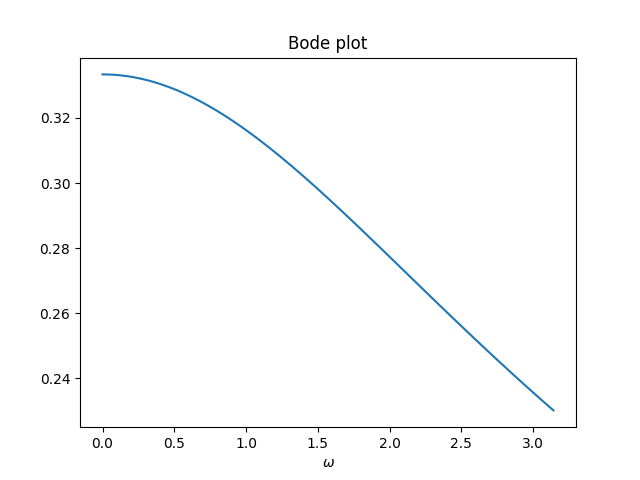
\includegraphics[width=0.95\textwidth]{figures/p3_bode.png}
    \end{center}
    \caption{Bode plot of system.}
\end{figure}

\subsection*{System output}
Let some input be defined as 
\begin{align}
    x(t) &= \begin{cases}
        e^{-t}, &\text{ if }t\geq 0\\
        0        
    \end{cases}\\ 
        &= e^{-t}u(t).
\end{align}

From earlier we know
\begin{align}
    H(j\omega) = \frac{1}{3 + j\omega}
\end{align}

Then using table 4.2 from the book:
\begin{align}
    h(t) &= e^{-3t}u(t)\\
\Rightarrow y(t) &= h(t)*x(t)\\ 
    &= \int_\mathbb{R}d\lambda \ \ h(\lambda)x(t-\lambda)\\ 
    &= \int_\mathbb{R}d\lambda \ \ e^{-3\lambda}u(\lambda)
        e^{-(t-\lambda)}u(t-\lambda)\\ 
    &= \int_0^\infty d\lambda \ \ e^{-3\lambda}
        e^{-(t-\lambda)}\underbrace{u(t-\lambda)}
        _{\text{$t$ must be $\geq \lambda$}}\\ 
\end{align}

Note that $t\geq 0$, otherwise would this also give 0, as $\lambda$ needs to 
be greater or equal to 0, and $t$ must be greater than or equal to $\lambda$ 
due to the step functions. Hence
\begin{align}
    y(t)&= u(t)\int_0^t d\lambda \ \ e^{-3\lambda}e^{-(t-\lambda)}\\
    &= u(t)\int^t_0 d\lambda \ \ e^{-2\lambda - t} \\
    &= u(t)e^{-t}\int_0^td\lambda \ \ e^{-2\lambda}\\ 
    &= -u(t)\left[\frac{e^{-2(t + \lambda)}}{2}\right]_0^t\\ 
    &= \frac{e^{-t} - e^{-3t}}{2}u(t).
\end{align}
